\chapter{Learning to play connect four with RL}
\label{ch:connect_four_rl}
% The report should introduce the problem you solve and the algorithms you use.
% Your solution (with formulas and/or pseudocode)

The previous chapters introduced the main concepts of \glsfirst{rl} and \glsfirst{marl}.
It was discussed that real-life use cases for \gls{rl} are mostly limited to institutions with a high amount of resources at the moment.
As a possible use case for indie developers, which are small game companies or even individuals, the feasibility of using \gls{rl} as a computer opponent in the simple Python games was studied.
In particular, an open-source Pygame implementation of connect four was converted to a Gym-like environment and common \gls{rl} algorithms were trained in an online manner on it.
This chapter highlights the design decisions of that systems.
All of the documented source code together with annotated Jupyter Notebooks are available on the GitHub repository of this project \citep{github_project}.

%------------------------------------

\section{Connect four and its complexity}
\label{sec:connect_four_rl-harder_then_you_think}

Connect four is a trademarked game first sold in February 1974, although many similar connection board games have been made throughout history.
In connect four, two players compete against each other by dropping player-specific coins into an open slot of a shared board.
This board is seven columns wide and six rows high.
A player drops a coin from the top of a column and it drops to the lowest available row of that column which still has a free spot.
If there is no free spot in a specific column, the coin can not be inserted in that column.
The game is won by the player that can connect four of their pieces in a straight horizontal, vertical or diagonal line.
When to board is full and none of the players has won, the game is a tie. 
A sample game between a rainbow policy and human player is shown in Figure \ref{fig:rainbow_diagonal_win_turn_annotation}, a video of which is also available on YouTube \footnote{\url{https://youtube.com/shorts/DZesQ4GI0hE}}.

The rules of connect four are very simple and with a board of only six by seven, the game seems simple enough.
However, connect four has $4531985219092$ possible boards, which is in the order of $\approx 10^{13}$.
Whilst this is still far less than the game complexity of chess ($\approx 10^{123}$) or Go ($\approx 10^{360}$), it is still significantly larger than the simple rules would suggest.
Since there are so many states, each with up to seven possible actions (free columns), tabular approaches as discussed in section \ref{sec:intro-approaches} are not feasible.
Not only would such a table require significant memory, but it would also take far too long to reach all states at least once.
This further shows how limited tabular methods are.

Whilst a manual feature representation could potentially be determined that lowers the state dimension to a feasible amount, it would require a domain specific approach and would give no value to a general feasibility study.
Because of this, a \glsfirst{drl} approach is taken to learn the connect four game.
This will make it possible to learn directly from the matrix representation of the board shown in the annotations of Figure \ref{fig:intro_rl_cycle}.
Two \glsfirst{dqn} approaches and one Rainbow approach are implemented and trained in a variety of ways, which is discussed in what follows.


\begin{figure}[ht]
    \centering
    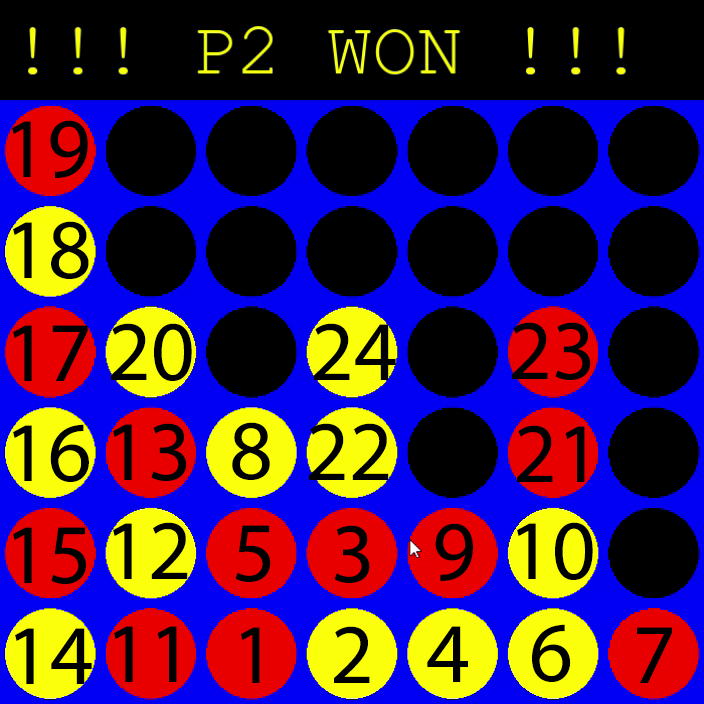
\includegraphics[width=0.7\linewidth]{images/ConnectZero_rainbow_diag_human_win.png}
    \captionsetup{width=0.9\linewidth}
    \captionsetup{justification=centering}
    \caption{Sample connect four game annotated with the time steps at which the coins are placed. Player one is red and is the best-found rainbow policy from the paper notebook 9, player two is yellow and is a human. Player two won with the diagonal coins of 14, 12, 8 and 24.  A video of this game can be found on YouTube (\url{https://youtube.com/shorts/DZesQ4GI0hE}).}
    \label{fig:rainbow_diagonal_win_turn_annotation}
\end{figure}

%------------------------------------

\section{Gym implementation of connect four game environment}
\label{sec:connect_four_rl-gym-environment}


Since this paper aims to study the feasibility of implementing \gls{rl} opponents in simple Python based games, it was chosen to build further upon an existing connect four implementation.
The chosen base implementation is one by \citet{base_connectfour_github} and makes use of the popular Pygame library by \citet{pygame}.
The author's permission of reusing his code was granted after brief communication on LinkedIn.
Some edits were made to this base implementation to make the code more readable and the game UI more informative. 
Since this base game is just a human-play variant of the connect four game, it lacks many of the components required to use it in a \gls{rl} setting such as a reward strategy and more.

As a first step of converting this base Pygame to an environment usable for \gls{marl}, it was converted to a custom Gym environment.
A custom Gym environment should inherit from the Gym class and provide a few specific attributes and functions, a skeleton for this is given in Algorithm \ref{alg:minimal_gym_structure}.
A Gym environment is a class from the popular Gym library by \citet{gym} introduced in section \ref{sec:intro-classical_rl}.
Converting the base Pygame to a Gym environment was straightforward given the many tutorials and documentation available discussing how to create a custom environment.
The conversion process took about four hours, including testing.
This version of the environment is called \texttt{ConnectFourPygameEnvV1} and is available under \texttt{gym\_connect4\_pygame} folder in the Github repository of this project \citep{github_project}. 

The init method supports two render modes, \texttt{terminal} and \texttt{human}.
It also allows for specifying the column and row count of the connect four board, although the default grid of 6x7 is used throughout this paper.
The observation space is specified as a Gym directory consisting of one key called \texttt{board}.
The board in the observation space is a two-dimensional Gym box ($\approx$ 2D array) with integer values between zero and two, including boundaries.
Zero corresponds to an empty space, 1 to the first player's coin and 2 to the second player's coin.
This corresponds to the representation annotated in Figure \ref{fig:intro_rl_cycle}.
The action space is a discrete space specifying an integer that corresponds to the column index a coin should be dropped into.

The step method contains the main logic of a Gym environment as it performs a specified action in the environment and updates the state of the environment.
It also returns a reward, a boolean to specify if the game has ended and an info object.
In this implementation, there is no mechanism in place to reject a player to insert a coin in a full column.
However, attempting to do so keeps the board unaltered and gives the turn to the same player again.
After this, the step function checks for a winning board or tie board to end the game.
If the game is not over, the step function alternates the current player.
The step function makes use of many abstracted functions from the base game, which are not shown in the minimal Gym skeleton of Algorithm \ref{alg:minimal_gym_structure}.

The render method supports a terminal printed render of the board which prints the 2D matrix representation of the board after each step.
It also has support for a human mode which renders the game in a Pygame instance, just like playing the game regularly would do.
The reset and close functions are trivial and are not discussed in detail. 
The experimental notebook 2 gives details on how to work with this V1 of the custom connect four Gym environment \citep{github_project}.
Since the Gym environment doesn't provide any standards on specifying a multi-agent environment, the implementation is custom and does not comply with any specific standard.
In essence, the info object, which is one of the returned values from the step and reset function, gives all the required info for playing a loop in the game.
Since this custom Gym environment is multi-agent but doesn't follow any conventions, it is not supported directly by any \gls{rl} algorithm library and is therefore not used.

\begin{algorithm}
    \caption{Minimal structure of a Gym environment}
    \Comment{Init method should accept a render mode.}
    \Function{\_\_init\_\_(self, render\_mode, ...)}{
        \If{$\var{loss} > \theta_{\mathrm{exp}}$} {
            ... \;
            \Comment{Observation space for the environment: structure of an observation}
            self.observation\_space = gym.spaces.Dict(...)\;
            ...\;
            \Comment{Action space for the environment: structure for an action}
            self.action\_space = gym.spaces.Discrete(...)\;
            ...\;
        }
    }
    \Comment{Reset function to return the environment to its start state.}
    \Function{reset(self, return\_info=False)}{
        ...
        \Return{(observation, info) if return\_info else observation}\;
    }
    \Comment{Step function to perform an action in the environment.}
    \Function{step(self, action: int)}{
        ...\;
        \Comment{Return an observation of the new state, the received reward, a boolean specifying if the environment is finished and an info object containing additional information.}
        \Return{observation, reward, done, info}\;
    }
    \Comment{Render function to visualise the environment.}
    \Function{render(self, mode='terminal')}{
        ...
        
    }
    \Comment{Close function to clean up an environment.}
    \Function{close(self)}{
        ...
    }
    \label{alg:minimal_gym_structure}
\end{algorithm}

%------------------------------------

\section{Petting Zoo implementation of connect four}
\label{sec:connect_four_rl-pettingzoo-environment}
% TODO: dit blokje is klaar maar brakka spelling, herlees and grammarly

Having implemented the base game as a custom Gym environment, it was concluded that such a custom multi-agent Gym environment which doesn't follow any conventions doesn't neatly integrate with existing \gls{rl} algorithm libraries such as Tianshou \citep{tianshou} and Ray RLlib \citep{rllib}.
As this paper is a feasibility study, which includes ease of implementation as a criteria, it was opted to adopt this V1 of the environment to a Petting Zoo environment which is supported by these libraries.
As discussed in section \ref{sec:intro-classical_rl}, Petting Zoo is a commonly used library for \gls{marl} as it provides multi-agent environments in a Gym like manner.
Converting the Gym environment to a Petting Zoo based environment was not as trivial as going to a Gym environment from the base game.
This is mostly due to the Petting Zoo documentation not providing instructions on how to implement a custom environment, which the Gym library documentation did do.
However, through studying the source code of simple environments provided by Petting Zoo, such as the Tic-Tac-Toe environment, adopting the custom Gym environment to a Petting Zoo compatible environment was possible in about 10 hours of work.
Most of this time was spending time troubleshooting compatibility issues with the \gls{rl} algorithm library Tianshou that integrate directly with Petting Zoo environments.
This direct integration relied on the presence of some functions and wrappers which were not directly clear that they were needed from studying source code of other Petting Zoo environments. 

The Petting Zoo variant of the connect four game is provided as \texttt{ConnectFourPygameEnvV2} under the \texttt{gym\_connect4\_pygame} folder in the Github repository of this project \citep{github_project}.  
Most notable changes include inheriting from the Petting Zoo \texttt{AECEnv} class rather then Gym's \texttt{Env} class and wrapping this custom Petting Zoo environment in some common Petting Zoo environment wrappers. 
The observation space is also extended to include an action mask besides the board representation taken straight from the V1 variant of the environment.
This action masks specifies which of the actions from the action space are valid for the current state.
If specified during initialisation, the environment can thus strictly enforce an agent to only use an allowed action for a given state.
Whilst this incorporates some domain knowledge, it can drastically improve the learning speed of the agents.
However, it is still possible to let the agents learn this behaviour by specifying to not use the mask and giving a negative reward to placing a coin in a full column.
Besides this, the observation space and action space should be lists containing a variant of the space for both agents, although these spaces are equal for both agents in the connect four game environment.
Next to this, the \texttt{step} and \texttt{reset} method no longer return game information such as the state, done boolean, reward and info object.
Rather, Petting Zoo maintains variables such as \texttt{rewards}, \texttt{dones} and \texttt{infos} to keep track of the game state and has an \texttt{observe} function.
Exact implementation details are not of importance and thus not given in this paper, although the source code is documented and available on GitHub \citep{github_project}.

%------------------------------------

\section{Reward strategy}
\label{sec:connect_four_rl-rewards}
% reward for block etc -> https://openai.com/blog/competitive-self-play/

TODO

%------------------------------------

\section{Using MLP based deep Q-networks to learn connect four}
\label{sec:connect_four_rl-mlp-dqn}
% tekeningetje van de MLP?
% Short uitleggen wat DQN is

TODO

%------------------------------------

\section{Using CNN based deep Q-networks to learn connect four}
\label{sec:connect_four_rl-cnn-dqn}
% tekeningetje van de CNN?

TODO

%------------------------------------

\section{Using CNN based Rainbow to learn connect four}
\label{sec:connect_four_rl-dqn}
% ref tekeningtje CNN DQN want zelfde clue 
% Geen full uitleg geven en zeggen hoe dit mooi is gezien het implementation makkelijker maakt maar wel de basics geven

TODO

%------------------------------------

\section{Using MiniMax as a rule-based opponent}
\label{sec:connect_four_rl-minimax_opponent}
% Zeggen hoe minimax gewoon tree search is en dus geen RL maar wel gebruikt kan worden als fixed opponent zoals gezegd in section marl_opponents

TODO